\chapter{自旋、测量与二维态空间}

\lectureoverview{自旋具有方向性，然而对其任意一个分量的每一次测量都只返回\(+1\)或\(-1\)。我们首先表述这一操作层面的困惑，然后说明为什么普通的集合逻辑对不相容的测量失效。一个二维复矢量空间提供了恰当的语言：概率来自振幅，可区分的备选是正交的，而上--下、右--左、里--外三组基编码了三个空间方向，却不会把态矢量变成一支普通的箭头。}

\section{从量子比特到自旋}

先前作为量子比特引入的二态系统，现在将被称为\emph{自旋}。名称的改变把空间方向带入了讨论，但也在\emph{矢量}一词中造成了危险。必须把两个不同的对象区分开来：

\begin{definition}
\emph{三维矢量}是三维空间中的普通实矢量。不加限定的\emph{矢量}将指抽象矢量空间的一个元素，例如量子力学中使用的复态空间。
\end{definition}

自旋可以相对于普通空间中的某一轴来制备。然而，它的态将由一个抽象矢量表示。这两个陈述之间的关系正是我们必须去发现的事情之一；它不能从一幅图像中假定。

\section{为什么仪器不能被移除}

经典力学鼓励我们想象一位理想的观察者，他在了解一个系统的同时，能随心所欲地尽量少扰动它。例如，假设我们想看见一个宏观物体。我们照亮它，用透镜收集反射光，并放大图像。光会施加一定的力，但在经典理想化中，其强度可以降低而放大倍数可以提高。扰动可以被做得任意小，而不必放弃测量的观念。

这一取极限的程序在量子力学中失效。仪器可以被改进、屏蔽和校准，但一般说来，测量不可能既提供信息又任意地不具侵入性。系统的某些东西发生了变化。这并不意味着每一次测量都破坏每一个性质，也不意味着结果不能被重现。它意味着仪器是被提出的物理问题的一部分，而测量之后的态不能被忽略。

目前，暂且把仪器看作一个具有两个特征的黑箱：它可以在空间中取向，其显示记录\(+1\)或\(-1\)。板上的小箭头是标记已制备自旋的方便记号：

\begin{figure}[htbp]
\centering
\includegraphics[width=0.64\textwidth]{lecture_02_figure_02.png}
\caption{沿某一轴制备的自旋的第一个临时标记。箭头标记的是一种制备；它还不是态的经典模型。}
\lectureframe{00:05:15}
\end{figure}

选择坐标轴，使\(z\)指向板上方，\(x\)指向右方，\(y\)指向板外。如果仪器沿单位方向\(\hat m\)取向，其结果为
\begin{equation}
\sigma_{\hat m}=\pm1.
\end{equation}
特别地，
\[
\sigma_z=\pm1,\qquad \sigma_x=\pm1,\qquad \sigma_y=\pm1.
\]
在这个阶段，\emph{分量}一词是操作性的：\(\sigma_z\)就是取向仪器沿\(z\)方向时报告的结果。它还不是某个隐藏的经典箭头的\(z\)分量。

\subsection{可重复性与扰动}

假设一次\(z\)测量给出\(+1\)。在没有中间操作的情况下，第二次\(z\)测量再次给出\(+1\)，进一步的重复也是如此。第一次测量已经制备了一个态，在其中同一个问题有确定的答案。

\begin{classroomqa}
\audiencequestion{如果量子测量扰动了自旋，为什么立即重复会返回相同的结果？}
\lecturerresponse{扰动并非不加区分。测量\(\sigma_z\)可以改变以后\(x\)或\(y\)测量中将会发生的事，同时使新测得的\(\sigma_z\)值保持可重复。一个有用的实验恰恰需要这种有限形式的稳定性。}
\end{classroomqa}

现在把仪器转过\(180^\circ\)。一个在朝上取向时给出\(+1\)的自旋，在倒转取向下给出\(-1\)。再把仪器转回朝上，结果又是\(+1\)。因此取向很重要。温度计不会仅仅因为被倒过来就报告负的温度；自旋分析器行为不同，是因为它问的是一个有方向性的问题。

\begin{figure}[htbp]
\centering
\includegraphics[width=0.72\textwidth]{lecture_02_figure_03.png}
\caption{板上记录着二值标记\(\sigma_z=\pm1\)和\(\sigma_x=\pm1\)，以及\(x\)轴提示。}
\lectureframe{00:12:46}
\end{figure}

与经典单位矢量的对比是直接的。经典分量在\(-1\)与\(+1\)之间连续变化。垂直于\(x\)轴的单位矢量，其\(x\)分量为零。相反，沿\(x\)方向指向的自旋分析器从不显示零。它显示\(+1\)或\(-1\)，即使自旋是沿\(z\)方向制备的。

\section{单一结果与类矢量平均值}

通过获得\(\sigma_z=+1\)来制备一个自旋，然后测量\(\sigma_x\)。在相同制备的试验中，一半给出\(+1\)，一半给出\(-1\)。因此
\begin{equation}
\langle \sigma_x\rangle=0.
\end{equation}
同样的制备给出
\begin{equation}
\langle \sigma_y\rangle=0.
\end{equation}
反之，以\(\sigma_x=+1\)制备的自旋，在随后的\(z\)或\(y\)测量中，两个结果具有相等的概率。

这句话中隐藏着两个不同的实验。在第一次\(x\)结果之后，对\emph{同一}自旋反复测量\(\sigma_x\)，仅仅确认了那个结果。要获得五五--开的统计，需要许多制备在同一\(z\)态的自旋，或者一个自旋在每次\(x\)测量之前反复回到同一制备。

\begin{classroomqa}
\audiencequestion{如果一个自旋在进入装置之前没有被有意制备，会发生什么？}
\lecturerresponse{结果仍然是\(+1\)或\(-1\)，但其概率取决于自旋实际具有的状态。制备是使重复试验可比较的受控程序。如果在两次测量之间发生了未知的操作，可重复性就不再得到保证；如果没有发生任何事情，同分量的结果就是可重现的。}
\end{classroomqa}

\subsection{两个任意方向}

通过从沿\(\hat n\)方向取向的分析器获得\(+1\)，将自旋制备在单位方向\(\hat n\)上。然后沿另一个单位方向\(\hat m\)进行测量。每次试验仍然只给出\(\pm1\)，但在相同制备的试验上的平均值为
\begin{equation}
\boxed{\langle\sigma_{\hat m}\rangle=\hat n\cdot\hat m
=\cos\theta_{nm}.}
\label{eq:spin-average}
\end{equation}
板书使用更简短的记号\(\langle\sigma_m\rangle=n\cdot m\)：

\begin{figure}[htbp]
\centering
\includegraphics[width=0.74\textwidth]{lecture_02_figure_04.png}
\caption{类矢量的规律属于系综平均值，而不属于单个\(\pm1\)结果。}
\lectureframe{00:23:22}
\end{figure}

方程~\eqref{eq:spin-average}包含了先前的情况。如果\(\hat m=\hat n\)，平均值为\(+1\)；由于没有结果能超过\(+1\)，每次试验都给出\(+1\)。如果\(\hat m=-\hat n\)，每次试验都给出\(-1\)。垂直的轴给出零平均值和相等的频率。

如果\(p_+\)和\(p_-\)表示两个可能结果的概率，那么
\[
p_++p_-=1,\qquad p_+-p_-=\hat n\cdot\hat m.
\]
因此，
\begin{equation}
p_\pm=\frac{1\pm\hat n\cdot\hat m}{2}.
\label{eq:direction-probabilities}
\end{equation}
\editorialnote{讲座陈述了两个结果及其平均值。方程~\eqref{eq:direction-probabilities}是这两个事实的直接代数推论。}

\begin{classroomqa}
\audiencequestion{尖括号中的量是\emph{期望值}还是普通平均值？}
\lecturerresponse{它是许多次重复中记录结果的平均值。\emph{期望值}是标准术语，但这里并不意指任何额外类型的平均。装置产生一个由\(+1\)和\(-1\)组成的列表；尖括号表示在大系综极限下该列表的算术平均。}
\end{classroomqa}

\begin{classroomqa}
\audiencequestion{在平均值规律已知之前，箭头\(\hat n\)是否已经具有几何意义？}
\lecturerresponse{最初它只是制备装置如何取向的标签。反转实验以及平均值对\(\hat n\cdot\hat m\)的依赖赋予该标签操作性的几何意义。装置定义了分量的含义；单个结果从不提供经典投影。}
\end{classroomqa}

这是方向性图像与离散数据的第一次调和。单个自旋的行为并不像具有连续取值分量的经典箭头。然而，许多相同制备的自旋的统计性质，其变换方式恰好与单位三维矢量的分量相同。

\section{经典命题作为集合}

在构造量子态空间之前，先考虑逻辑对经典系统如何运作。设可能的状态构成一个集合\(\Omega\)。命题\(A\)由使\(A\)为真的状态子集表示。

对于一个六面骰子，
\[
A=\{2,4,6\}
\]
可以表示\emph{结果为偶数}，而
\[
B=\{4,5,6\}
\]
可以表示\emph{结果大于三}。逻辑运算变为集合运算：
\begin{equation}
\neg A=A^c,\qquad
A\land B=A\cap B,\qquad
A\lor B=A\cup B.
\label{eq:classical-logic}
\end{equation}
这里\(\lor\)是包含或：当\(A\)为真、\(B\)为真，或两者都为真时，\(A\lor B\)为真。它不是日常用语中排他的\emph{要么\(A\)要么\(B\)，但不同时成立}。

\begin{classroomqa}
\audiencequestion{自旋测量只有两个结果，但制备方向连续变化。态集合是有限的还是连续的？}
\lecturerresponse{可能的制备方向集合是连续的，尽管每个选定的分析器只有两个读数。这正是为什么仅靠计数探测器标签不足以描述态空间。}
\end{classroomqa}

对于经典子集，交和并不关心哪个命题先被提及：
\[
A\cap B=B\cap A,\qquad A\cup B=B\cup A.
\]
因此，对经典复合命题的实验检验可以在不把顺序引入逻辑的情况下被理想化。

\section{一个依赖顺序的或检验}

考虑量子命题
\begin{equation}
A:\sigma_z=+1,\qquad B:\sigma_x=+1.
\end{equation}
每个命题都有一个明确的检验。将装置沿\(z\)方向取向以检验\(A\)，或沿\(x\)方向取向以检验\(B\)。当人们试图通过检验一个命题、若其为假则检验另一个命题来验证\(A\lor B\)时，麻烦就出现了。

设想一位看不见的制备者提供了一个\(z\)向上的自旋。如果先检验\(A\)，结果必然是\(+1\)，或检验以\emph{真}结束。

颠倒顺序。先检验\(B\)给出
\[
P(B)=\frac12,\qquad P(\neg B)=\frac12.
\]
如果\(B\)为假，\(x\)测量 nevertheless 制备了一个确定的\(x\)态。在该态上检验\(A\)给出
\[
P(A\mid \neg B)=\frac12,\qquad
P(\neg A\mid \neg B)=\frac12.
\]
因此，颠倒后的程序以概率
\begin{equation}
P(\neg B\ \text{then}\ \neg A)
=\frac12\cdot\frac12=\frac14.
\end{equation}
报告两个命题都为假。一种顺序总是接受或；另一种在四分之一的试验中拒绝它。

\begin{classroomqa}
\audiencequestion{这一矛盾仅仅是由我们对秘密制备态的知识不完整造成的吗？}
\lecturerresponse{不是。隐藏的制备只是为了使命题比较变得清晰。第一次\(x\)测量在物理上制备了一个\(x\)态，因此后来的\(z\)检验是在一个已改变的态上进行的。给观察者更多关于初始制备的信息并不能撤销那次干预。}
\end{classroomqa}

\begin{classroomqa}
\audiencequestion{能否通过更精细的问题层级而不是这种顺序规则来检验或？}
\lecturerresponse{当然可以定义不同的实验程序，但那样它们就是不同的量子测量。不存在一个与程序无关的子集\(A\cup B\)，其真值可以简单地被揭示而不考虑装置。顺序依赖是一个警告：经典集合逻辑不是这些命题的固有逻辑。}
\end{classroomqa}

稍后，命题将由投影算符表示。简洁的代数警告是
\begin{equation}
P_A P_B\ne P_B P_A.
\end{equation}
目前还不需要算子理论的更多内容。重要的是，不相容的检验不对易，它们的复合命题不能当作普通的集合并来处理。

\begin{classroomqa}
\audiencequestion{能否安排这个实验的双粒子版本，使得检验的选择在时间上向后作用？}
\lecturerresponse{这个问题需要这里尚未发展的机制。从单自旋序列不能得出关于反向因果的结论，因此该问题被留作未决，而不是加以猜测。}
\end{classroomqa}

\section{线性态空间}

集合包含元素，但通常没有自然的方式将两个元素相加得到第三个。线性向量空间有更多的结构。如果\(\ket{A}\)和\(\ket{B}\)是向量且\(\alpha,\beta\in\mathbb C\)，那么
\begin{equation}
\alpha\ket{A}+\beta\ket{B}
\end{equation}
是同一空间中的另一个向量。量子态在这样的复线性空间中表示。

对于每个右矢\(\ket{A}\)，都有一个对应的对偶左矢\(\bra{A}\)。将左矢与右矢配对得到一个复数，即内积。它满足共轭对称性，
\begin{equation}
\braket{A}{B}=\braket{B}{A}^{*}.
\label{eq:conjugate-symmetry}
\end{equation}

\begin{figure}[htbp]
\centering
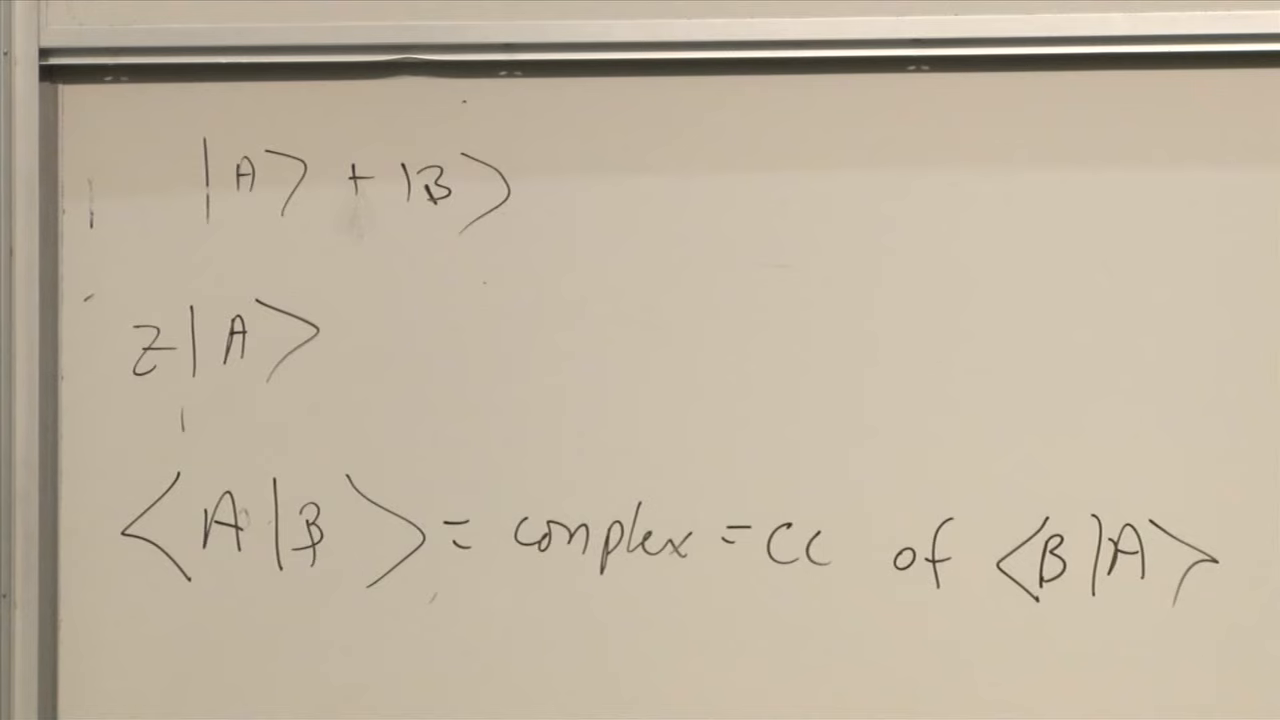
\includegraphics[width=0.78\textwidth]{lecture_02_figure_05.png}
\caption{板书总结了线性组合和内积的共轭反转。}
\lectureframe{00:46:53}
\end{figure}

向量的长度平方为
\begin{equation}
\|\ket{A}\|^2=\braket{A}{A}.
\end{equation}
方程~\eqref{eq:conjugate-symmetry}使这个数等于它自己的复共轭，因此是实数；内积的公理也使它非负。当
\begin{equation}
\braket{A}{B}=0.
\end{equation}
时，两个向量正交。空间的维数是所能选取的相互正交的非零方向的最大数目。

\begin{classroomqa}
\audiencequestion{是否每个基都必须由相互正交的矢量组成？}
\lecturerresponse{不是。基只需线性无关且张成该空间。正交基特别方便，因为系数和概率容易提取。在二维中，两个不平行矢量即使内积不为零，也可以构成一组基。}
\end{classroomqa}

\section{二维自旋空间}

一个自旋的状态空间被假定为二维复矢量空间，
\begin{equation}
\mathcal H_{\mathrm{spin}}\cong\mathbb C^2.
\end{equation}
存在连续无穷多个可能的状态矢量，但只需两个独立的基矢量即可表示其中任何一个。

从由沿\(z\)方向取向的装置制备的状态开始：
\begin{align}
\ket{u}&\longleftrightarrow \sigma_z=+1,\\
\ket{d}&\longleftrightarrow \sigma_z=-1.
\end{align}
字母\(u,d\)、符号\(+,-\)和箭头\(\uparrow,\downarrow\)是同一对制备的替代标记。由于\(z\)测量能确定地将它们区分开，它们的态矢量正交：
\begin{equation}
\braket{u}{d}=0.
\end{equation}
选择它们具有单位长度，
\[
\braket{u}{u}=\braket{d}{d}=1.
\]

于是每个自旋态都可写成
\begin{equation}
\ket{A}=\alpha_u\ket{u}+\alpha_d\ket{d},
\qquad \alpha_u,\alpha_d\in\mathbb C.
\label{eq:general-spin-state}
\end{equation}
概率规则为
\begin{equation}
P(u|A)=|\alpha_u|^2,\qquad
P(d|A)=|\alpha_d|^2.
\label{eq:born-z}
\end{equation}
因为两个结果之一必然发生，
\begin{equation}
|\alpha_u|^2+|\alpha_d|^2=1.
\label{eq:normalization}
\end{equation}

\begin{figure}[htbp]
\centering
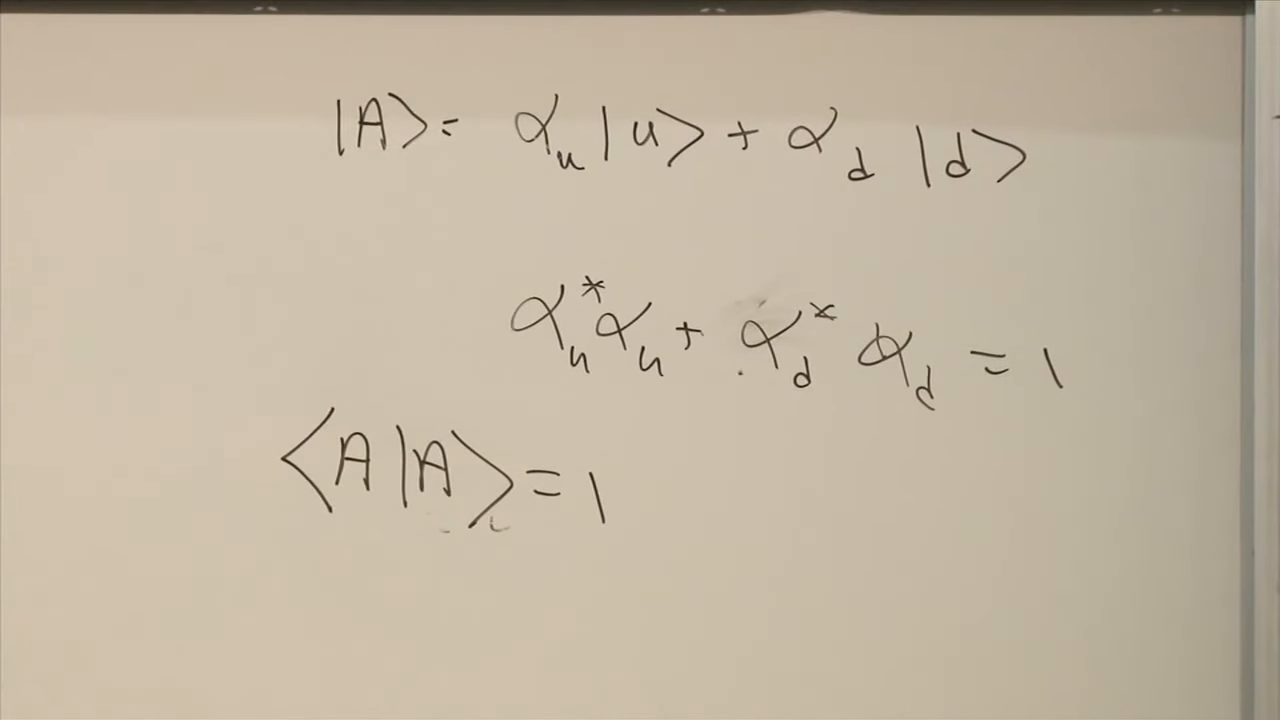
\includegraphics[width=0.78\textwidth]{lecture_02_figure_06.png}
\caption{一般的上--下展开、两个结果概率之和，以及等价的单位范数条件。}
\lectureframe{01:03:38}
\end{figure}

与单位归一化的等价性直接可得：
\begin{align}
\braket{A}{A}
&=(\alpha_u^*\bra{u}+\alpha_d^*\bra{d})
  (\alpha_u\ket{u}+\alpha_d\ket{d})\\
&=|\alpha_u|^2\braket{u}{u}
 +\alpha_u^*\alpha_d\braket{u}{d}\\
&\quad +\alpha_d^*\alpha_u\braket{d}{u}
 +|\alpha_d|^2\braket{d}{d}\\
&=|\alpha_u|^2+|\alpha_d|^2=1.
\end{align}
因此，物理纯态由归一化矢量表示。

\begin{classroomqa}
\audiencequestion{这些陈述是被推导出来的，还是公设？}
\lecturerresponse{在这一点上，它们是被用来拟合实验的规则。二维空间、概率规则以及正交性的解释都是启发式地引入的。它们之间的相互一致性现在可以检验；状态与可观测量之间的系统关系将在接下来讨论。}
\end{classroomqa}

\subsection{正交性作为可区分性}

正交性的物理内容比垂直箭头的图像更有用：

\begin{quote}
能被一次测量确定地区分开的状态由正交矢量表示。
\end{quote}

上和下满足这一判据。如果状态为上，则\(z\)装置绝不会报告下，反之亦然。非零重叠表明，一个状态有时能产生与另一个状态相关联的结果。

\section{右--左基}

设\(\ket{r}\)和\(\ket{l}\)表示具有确定\(x\)自旋的态：
\[
\ket{r}\longleftrightarrow\sigma_x=+1,\qquad
\ket{l}\longleftrightarrow\sigma_x=-1.
\]
因为空间是二维的，每个态都必须是\(\ket{u}\)和\(\ket{d}\)的线性组合。沿右方向制备的自旋给出上和下的概率相等，因此两个系数的模必须相等。选择最简单的相位约定：
\begin{equation}
\ket{r}=\frac{1}{\sqrt2}\bigl(\ket{u}+\ket{d}\bigr).
\label{eq:right-state}
\end{equation}
右和左能被\(x\)装置确定地区分开，因此左态必须与右态正交。一个方便的选择是
\begin{equation}
\ket{l}=\frac{1}{\sqrt2}\bigl(\ket{u}-\ket{d}\bigr).
\label{eq:left-state}
\end{equation}
确实，
\begin{align}
\braket{l}{r}
&=\frac12(\bra{u}-\bra{d})(\ket{u}+\ket{d})\\
&=\frac12(1-1)=0.
\end{align}

\begin{figure}[htbp]
\centering
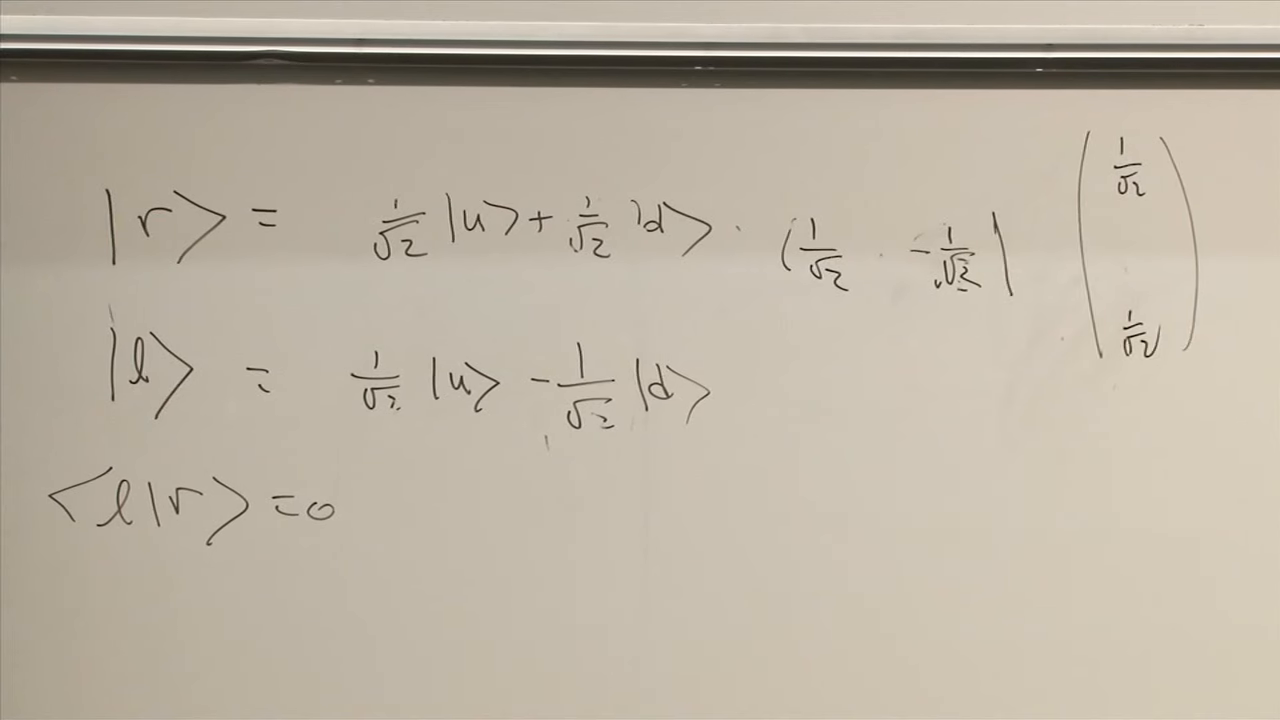
\includegraphics[width=0.82\textwidth]{lecture_02_figure_07.png}
\caption{完整的右--左构造：上--下模相等、相对符号相反，且内积为零。}
\lectureframe{01:12:15}
\end{figure}

\(\ket{l}\)的整体负号是约定性的。将\(\ket{l}\)替换为\(-\ket{l}\)不会改变其任何概率。将式~\eqref{eq:right-state}与式~\eqref{eq:left-state}相加和相减，得到逆基变换：
\begin{align}
\ket{u}&=\frac{1}{\sqrt2}\bigl(\ket{r}+\ket{l}\bigr),\\
\ket{d}&=\frac{1}{\sqrt2}\bigl(\ket{r}-\ket{l}\bigr).
\end{align}
这种对称性很重要。从\(x\)基出发，上态或下态是右和左的等权叠加，正如右态或左态是上和下的等权叠加一样。

\section{内--外基与相对相位}

将装置沿\(y\)方向取向，垂直于板面。写出
\[
\ket{i}\longleftrightarrow\sigma_y=+1,\qquad
\ket{o}\longleftrightarrow\sigma_y=-1,
\]
其中右矢标记\(i\)表示\emph{内}，而乘在右矢前的无附加标记的\(i\)仍是虚数单位。

上和下的概率相等要求系数模相等。内与外之间的正交性要求一个相对相位，使其重叠为零。一个对称的选择是
\begin{align}
\ket{i}&=\frac{1}{\sqrt2}\bigl(\ket{u}+i\ket{d}\bigr),\\
\ket{o}&=\frac{1}{\sqrt2}\bigl(\ket{u}-i\ket{d}\bigr).
\label{eq:in-out-states}
\end{align}
在\((u,d)\)基中，六个态为
\begin{align}
\ket{u}&=\binom10,
&
\ket{d}&=\binom01,
\\
\ket{r}&=\frac1{\sqrt2}\binom11,
&
\ket{l}&=\frac1{\sqrt2}\binom1{-1},
\\
\ket{i}&=\frac1{\sqrt2}\binom1{i},
&
\ket{o}&=\frac1{\sqrt2}\binom1{-i}.
\end{align}

\begin{figure}[htbp]
\centering
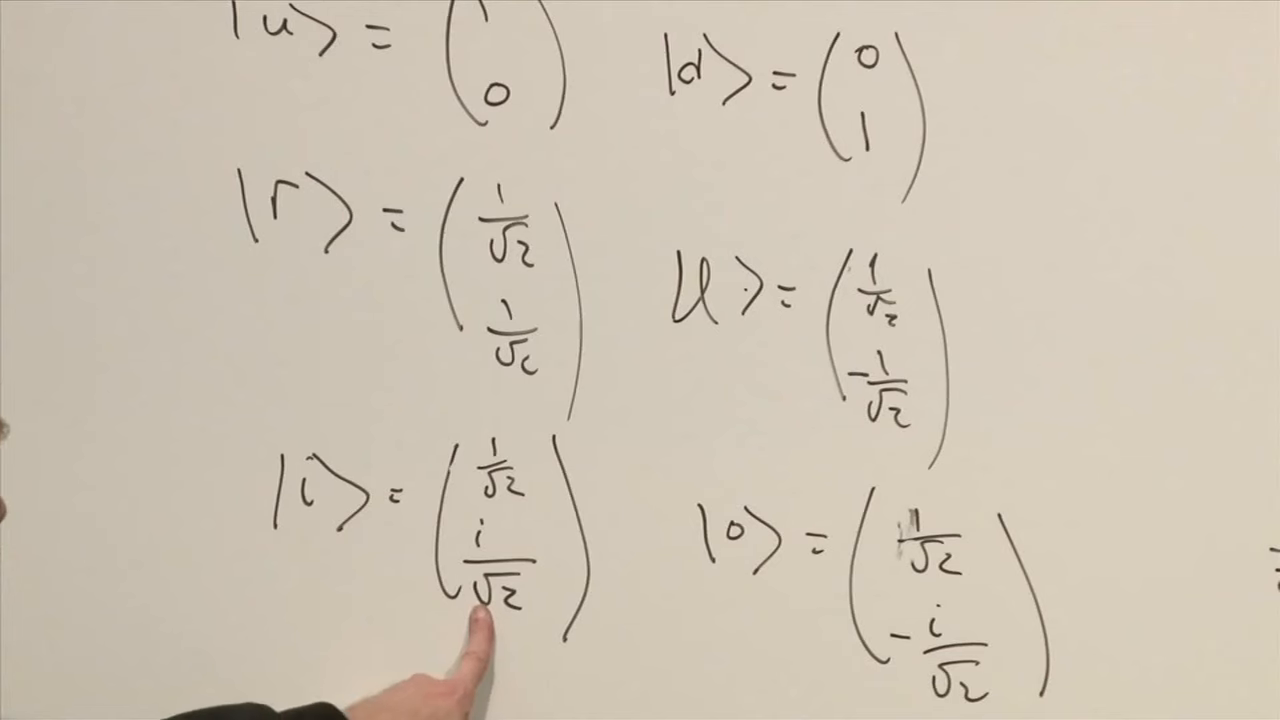
\includegraphics[width=0.82\textwidth]{lecture_02_figure_08.png}
\caption{上--下基中的六个列矢量。下面一对相差相对虚相位的符号。}
\lectureframe{01:20:50}
\end{figure}

左矢中的复共轭对于正交性检验至关重要：
\begin{align}
\braket{i}{o}
&=\frac12(\bra{u}-i\bra{d})(\ket{u}-i\ket{d})\\
&=\frac12\bigl(1+(-i)(-i)\bigr)=0.
\end{align}

\begin{classroomqa}
\audiencequestion{为\emph{in}选择\(+i\)而非为\emph{out}选择，是否编码了空间轴的手性？}
\lecturerresponse{一种约定已经引入，当泡利矩阵和旋转展开后，其几何意义将变得更加清楚。目前，这一对必须正交，并与其他基对称相关；交换标签或反转\(y\)轴改变的是约定，而不是构造的一致性。}
\end{classroomqa}

\subsection{在右--左基中检验对称性}

在入射态中使用
\[
\ket{u}=\frac{\ket{r}+\ket{l}}{\sqrt2},\qquad
\ket{d}=\frac{\ket{r}-\ket{l}}{\sqrt2}
\]：
\begin{align}
\ket{i}
&=\frac1{\sqrt2}
\left(
\frac{\ket{r}+\ket{l}}{\sqrt2}
+i\frac{\ket{r}-\ket{l}}{\sqrt2}
\right)\\
&=\frac{1+i}{2}\ket{r}
 +\frac{1-i}{2}\ket{l}.
\label{eq:in-in-rl}
\end{align}
尽管两个系数都没有明显包含\(1/\sqrt2\)，
\begin{equation}
\left|\frac{1+i}{2}\right|^2
=\left|\frac{1-i}{2}\right|^2
=\frac12.
\end{equation}

\begin{figure}[htbp]
\centering
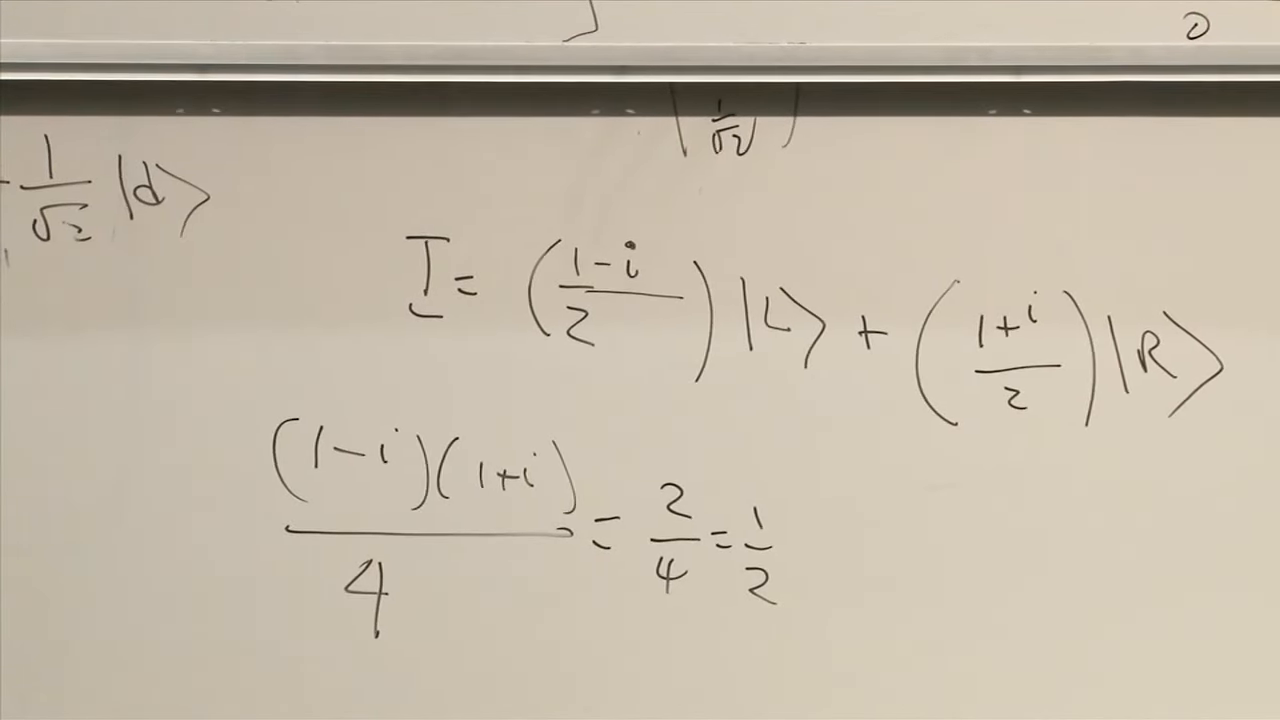
\includegraphics[width=0.82\textwidth]{lecture_02_figure_09.png}
\caption{入射态的实时基变换，以及每个右--左概率均为\(1/2\)的检验。}
\lectureframe{01:29:10}
\end{figure}

因此，三个基中任一基的每个态，在另外两个基中任一基测量时都给出相等概率。\(z\)、\(x\)和\(y\)基彼此互不偏倚。

\section{为什么有三对特殊的基}

\begin{classroomqa}
\audiencequestion{是否存在第四对态，与这三对态之间的对称关系相同？}
\lecturerresponse{对于单个二态系统，不存在。一旦三对互相无偏的态被固定，就不存在具有相同等重叠关系的第四对。存在三个这样的空间标签这一事实，与普通空间的三维性相关，尽管复态空间本身的维数是二。}
\end{classroomqa}

这一联系可以通过计数物理参数看出。一般的列
\[
\binom{\alpha_u}{\alpha_d}
\]
包含两个复数，因此有四个实数。归一化去掉一个：
\[
|\alpha_u|^2+|\alpha_d|^2=1.
\]
将两个分量乘以一个公共相位不改变任何测量概率：
\begin{equation}
\ket{A}\sim e^{i\chi}\ket{A}.
\label{eq:global-phase}
\end{equation}
这又去掉一个实参数。因此
\begin{equation}
4-1-1=2
\end{equation}
剩下物理实参数，恰好是指定三维空间中一个方向所需的角数。

一个方便的代表使这一关系变得明确：
\begin{equation}
\ket{\psi(\theta,\phi)}
=\cos\frac{\theta}{2}\,\ket{u}
+e^{i\phi}\sin\frac{\theta}{2}\,\ket{d}.
\label{eq:bloch-parameterization}
\end{equation}
\editorialnote{方程~\eqref{eq:bloch-parameterization}是讲座所确定的两参数族的标准归一化代表。显式的半角形式是为了使参数计数具体化；其动力学和旋转解释属于后续讲座。}

\begin{classroomqa}
\audiencequestion{忽略整体相位的精确数学是什么？}
\lecturerresponse{圆\(\{e^{i\chi}\ket{\psi}\}\)上的所有归一化矢量代表同一物理态。人们将这些矢量视为等价，就像由已声明的冗余相关联的点被视为一个物理点一样。分量之间的相对相位仍然可测量；只有乘以整个矢量的相位被丢弃。}
\end{classroomqa}

\begin{classroomqa}
\audiencequestion{未归一化的矢量或具有负分量的矢量是否仍可出现在计算中？}
\lecturerresponse{可以。线性代数允许它们，中间矢量不必已经代表制备好的物理态。非零矢量可以在最后归一化。负分量和复分量是振幅，不是负概率；概率来自态归一化后模的平方。}
\end{classroomqa}

\begin{classroomqa}
\audiencequestion{这一图像在更高维空间或更复杂的旋量中会变成什么？}
\lecturerresponse{同样的线性原理继续适用，但态空间维数、空间旋转和可观测自旋之间的关系变得更加丰富。这一推广超出了当前的二态构造。}
\end{classroomqa}

\section{正交性不是空间垂直性}

\emph{正交}一词现在带有抽象的、操作性的含义。它不能与普通空间中画出的两个箭头之间的夹角相混淆。空间方向上和下是相反的，但态矢量\(\ket{u}\)和\(\ket{d}\)是正交的。空间方向上和右是垂直的，然而
\begin{equation}
\braket{u}{r}=\frac1{\sqrt2}\ne0.
\end{equation}

\begin{classroomqa}
\audiencequestion{相反的空间方向如何能正交，而垂直的空间方向却不能？}
\lecturerresponse{态空间重叠度量的是实验可区分性，而不是标签之间的欧几里得角。上和下可以通过一次\(z\)测量确定地区分，因此它们的重叠为零。上和右则不能：一个沿右制备的自旋有时会给出上的结果。因此它们的态矢量有重叠。}
\end{classroomqa}

同样的思想在经典概率论中也有对应。两个支撑集不相交的概率分布是完全可区分的：观测到的结果就能确定使用的是哪一个分布。支撑集有重叠的分布则无法仅凭一次采样而无误差地区分。量子正交性扮演了不重叠的角色，而非零内积则表明某些结果与两种制备方式都相容。

\begin{classroomqa}
\audiencequestion{是否应当把二维态空间想象为包含向上箭头和向右箭头的物理平面？}
\lecturerresponse{不是。标记\(x,y,z\)指的是普通空间中仪器的取向。右矢属于一个带有自身内积的复向量空间。参数计数把这两种结构联系起来，但若把它们的图像逐点等同起来，就会把空间中的垂直与态空间中的正交混为一谈。}
\end{classroomqa}

\section{态、测量以及尚待完成的工作}

迄今为止，这一构造是通过让向量去拟合操作事实而推进的。三种仪器取向标记了三对归一化态，而它们之间的重叠则再现了观测到的概率。严格的处理仍须说明，诸如\(\sigma_z\)这样的可观测量如何作用于一个态，以及为什么它可能的结果就是它的本征值。这是下一步要做的事。

先前的逻辑谜题现在可以表述得更为尖锐。命题对应于子空间或它们的投影算符，而不相容的投影算符不对易。那个对顺序敏感的OR检验并不是一个言辞上的悖论；它是这种非对易结构的早期显现。

\begin{classroomqa}
\audiencequestion{如果态并不是一个普通的箭头，那么为什么三个标记\(x,y,z\)以及平均值\(\langle\sigma_{\hat m}\rangle\)看起来如此经典？}
\lecturerresponse{经典向量出现在系综平均中。单个自旋给出离散的答案，而许多以相同方式制备的自旋则给出像方向分量那样变换的平均值。当大量集合使这些平均值变得稳定时，宏观经典行为便涌现出来；不应反过来把它解读为每个单个自旋中隐藏着一个连续取值。}
\end{classroomqa}

\begin{classroomqa}
\audiencequestion{公共相位冗余是规范不变性的一个例子吗？}
\lecturerresponse{它是公共相位下的一种简单不变性，并预示了更广泛的规范思想。在这里展开这一联系会超出当前的构造，因此只保留物理上相关的陈述：公共相位不可见，相对相位则不然。}
\end{classroomqa}

最后，测量不应被想象为仅仅揭示出自旋一直以经典意义所携带的某个值。它制备出与所记录结果相关联的态。因此，立即重复同一次测量是相容的，而一組以相同方式制备的新自旋系综则显示出由相关振幅所决定的概率分布。一旦把可观测量作为算符引入，对这种制备与读出的数学描述就会变得精确。
